%╔════════════════════════════╗
%║	  Szablon dostosował	  ║
%║	mgr inż. Dawid Kotlarski  ║
%║		  06.10.2024		  ║
%╚════════════════════════════╝
\documentclass[12pt,twoside,a4paper,openany]{article}

    % ------------------------------------------------------------------------
% PAKIETY
% ------------------------------------------------------------------------
\usepackage{tikz}
\usepackage{./tikz-uml/tikz-uml}
\usepackage{float}

%różne pakiety matematyczne, warto przejrzeć dokumentację, muszą być powyżej ustawień językowych.
\usepackage{mathrsfs}   %Różne symbole matematyczne opisane w katalogu ~\doc\latex\comprehensive. Zamienia \mathcal{L} ze zwykłego L na L-transformatę.
\usepackage{eucal}      %Różne symbole matematyczne.
\usepackage{amssymb}    %Różne symbole matematyczne.
\usepackage{amsmath}    %Dodatkowe funkcje matematyczne, np. polecenie \dfac{}{} skladajace ulamek w trybie wystawionym (porównaj $\dfrac{1}{2}$, a $\frac{1}{2}$).

%język polski i klawiatura
\usepackage[polish]{babel}
%\usepackage{qtimes} % czcionka Times new Roman
\usepackage[OT4]{polski}
%\usepackage[cp1250]{inputenc}                       %Strona kodowa polskich znaków.

%obsługa pdf'a
\usepackage[pdftex,usenames,dvipsnames]{color}      %Obsługa kolorów. Opcje usenames i dvipsnames wprowadzają dodatkowe nazwy kolorow.
\usepackage[pdftex,pagebackref=false,draft=false,pdfpagelabels=false,colorlinks=true,urlcolor=blue,linkcolor=black,citecolor=green,pdfstartview=FitH,pdfstartpage=1,pdfpagemode=UseOutlines,bookmarks=true,bookmarksopen=true,bookmarksopenlevel=2,bookmarksnumbered=true,pdfauthor={Dawid Kotlarski},pdftitle={Dokumentacja Projektowa},pdfsubject={},pdfkeywords={transient recovery voltage trv},unicode=true]{hyperref}   %Opcja pagebackref=true dotyczy bibliografii: pokazuje w spisie literatury numery stron, na których odwołano się do danej pozycji.

%bibliografia
%\usepackage[numbers,sort&compress]{natbib}  %Porządkuje zawartość odnośników do literatury, np. [2-4,6]. Musi być pod pdf'em, a styl bibliogfafii musi mieć nazwę z dodatkiem 'nat', np. \bibliographystyle{unsrtnat} (w kolejności cytowania).
\usepackage[
	backend=biber,
	style=numeric,
	sorting=none
]{biblatex}
\addbibresource{bibliografia.bib}
\usepackage{hypernat}                       %Potrzebna pakietowi natbib do wspolpracy z pakietem hyperref (wazna kolejnosc: 1. hyperref, 2. natbib, 3. hypernat).

%grafika i geometria strony
\usepackage{extsizes}           %Dostepne inne rozmiary czcionek, np. 14 w poleceniu: \documentclass[14pt]{article}.
\usepackage[final]{graphicx}
\usepackage[a4paper,left=3.5cm,right=2.5cm,top=2.5cm,bottom=2.5cm]{geometry}

%strona tytułowa
\usepackage{strona_tytulowa}

%inne
\usepackage[hide]{todo}                     %Wprowadza polecenie \todo{treść}. Opcje pakietu: hide/show. Polecenie \todos ma byc na koncu dokumentu, wszystkie \todo{} po \todos sa ignorowane.
\usepackage[basic,physics]{circ}            %Wprowadza środowisko circuit do rysowania obwodów elektrycznych. Musi byc poniżej pakietow językowych.
\usepackage[sf,bf,outermarks]{titlesec}     %Troszczy się o wygląd tytułów rozdziałów (section, subsection, ...). sf oznacza czcionkę sans serif (typu arial), bf -- bold. U mnie: oddzielna linia dla naglowku paragraph. Patrz tez: tocloft -- lepiej robi format spisu tresci.
\usepackage{tocloft}                        %Troszczy się o format spisu trsci.
\usepackage{expdlist}    %Zmienia definicję środowiska description, daje większe możliwości wpływu na wygląd listy.
\usepackage{flafter}     %Wprowadza parametr [tb] do polecenia \suppressfloats[t] (polecenie to powoduje nie umieszczanie rysunkow, tabel itp. na stronach, na ktorych jest to polecenie (np. moze byc to stroma z tytulem rozdzialu, ktory chcemy zeby byl u samej gory, a nie np. pod rysunkiem)).
\usepackage{array}       %Ładniej drukuje tabelki (np. daje wiecej miejsca w komorkach -- nie są tak ścieśnione, jak bez tego pakietu).
\usepackage{listings}    %Listingi programow.
\usepackage[format=hang,labelsep=period,labelfont={bf,small},textfont=small]{caption}   %Formatuje podpisy pod rysunkami i tabelami. Parametr 'hang' powoduje wcięcie kolejnych linii podpisu na szerokosc nazwy podpisu, np. 'Rysunek 1.'.
\usepackage{appendix}    %Troszczy się o załączniki.
\usepackage{floatflt}    %Troszczy się o oblewanie rysunkow tekstem.
\usepackage{here}        %Wprowadza dodtkowy parametr umiejscowienia rysunków, tabel, itp.: H (duże). Umiejscawia obiekty ruchome dokladnie tam gdzie są w kodzie źródłowym dokumentu.
\usepackage{makeidx}     %Troszczy się o indeks (skorowidz).

%nieużywane, ale potencjalnie przydatne
\usepackage{sectsty}           %Formatuje nagłówki, np. żeby były kolorowe -- polecenie: \allsectionsfont{\color{Blue}}.
%\usepackage{version}           %Wersje dokumentu.

% 
\usepackage{csquotes}

%============
\usepackage{longtable}			%tabelka
%============

%============
% Ustawienia listingów do kodu
%============

\usepackage{listings}
\usepackage{xcolor}

\definecolor{codegreen}{rgb}{0,0.6,0}
\definecolor{codegray}{rgb}{0.5,0.5,0.5}
\definecolor{codepurple}{rgb}{0.58,0,0.82}
\definecolor{backcolour}{rgb}{0.95,0.95,0.92}

% Definicja stylu "mystyle"
\lstdefinestyle{mystyle}{
	backgroundcolor=\color{backcolour},
	commentstyle=\color{codegreen},
	keywordstyle=\color{blue},	%magenta
	numberstyle=\tiny\color{codegray},
	stringstyle=\color{codepurple},
	basicstyle=\ttfamily\footnotesize,
	breakatwhitespace=false,
	breaklines=true,
	captionpos=b,
	keepspaces=true,
	numbers=left,
	numbersep=5pt,
	showspaces=false,
	showstringspaces=false,
	showtabs=false,
	tabsize=2
}

\lstset{style=mystyle} % Deklaracja aktywnego stylu
%===========

%PAGINA GÓRNA I DOLNA
\usepackage{fancyhdr}          %Dodaje naglowki jakie się chce.
\pagestyle{fancy}
\fancyhf{}
% numery stron w paginie dolnej na srodku
\fancyfoot[C]{\scriptsize DOKUMENTACJA PROJEKTU – PROGRAMOWANIE URZĄDZEŃ MOBILNCH \\
	\normalsize\sffamily  \thepage}


%\fancyhead[L]{\small\sffamily \nouppercase{\leftmark}}
\fancyhead[C]{\footnotesize \textit{AKADEMIA NAUK STOSOWANYCH W NOWYM SĄCZU}\\}

\renewcommand{\headrulewidth}{0.4pt}
\renewcommand{\footrulewidth}{0.4pt}

    % ------------------------------------------------------------------------
% USTAWIENIA
% ------------------------------------------------------------------------ 

% ------------------------------------------------------------------------
%   Kropki po numerach sekcji, podsekcji, itd.
%   Np. 1.2. Tytuł podrozdziału
% ------------------------------------------------------------------------
\makeatletter
    \def\numberline#1{\hb@xt@\@tempdima{#1.\hfil}}                      %kropki w spisie treści
    \renewcommand*\@seccntformat[1]{\csname the#1\endcsname.\enspace}   %kropki w treści dokumentu
\makeatother

% ------------------------------------------------------------------------
%   Numeracja równań, rysunków i tabel
%   Np.: (1.2), gdzie:
%   1 - numer sekcji, 2 - numer równania, rysunku, tabeli
%   Uwaga ogólna: o otoczeniu figure ma być najpierw \caption{}, potem \label{}, inaczej odnośnik nie działa!
% ------------------------------------------------------------------------
\makeatletter
    \@addtoreset{equation}{section} %resetuje licznik po rozpoczęciu nowej sekcji
    \renewcommand{\theequation}{{\thesection}.\@arabic\c@equation} %dodaje kropki

    \@addtoreset{figure}{section}
    \renewcommand{\thefigure}{{\thesection}.\@arabic\c@figure}

    \@addtoreset{table}{section}
    \renewcommand{\thetable}{{\thesection}.\@arabic\c@table}
\makeatother

% ------------------------------------------------------------------------
% Tablica
% ------------------------------------------------------------------------
\newenvironment{tabela}[3]
{
    \begin{table}[!htb]
    \centering
    \caption[#1]{#2}
    \vskip 9pt
    #3
}{
    \end{table}
}

% ------------------------------------------------------------------------
% Dostosowanie wyglądu pozycji listy \todos, np. zamiast 'p.' jest 'str.'
% ------------------------------------------------------------------------
\renewcommand{\todoitem}[2]{%
    \item \label{todo:\thetodo}%
    \ifx#1\todomark%
        \else\textbf{#1 }%
    \fi%
    (str.~\pageref{todopage:\thetodo})\ #2}
\renewcommand{\todoname}{Do zrobienia\ldots}
\renewcommand{\todomark}{~uzupełnić}

% ------------------------------------------------------------------------
% Definicje
% ------------------------------------------------------------------------
\def\nonumsection#1{%
    \section*{#1}%
    \addcontentsline{toc}{section}{#1}%
    }
\def\nonumsubsection#1{%
    \subsection*{#1}%
    \addcontentsline{toc}{subsection}{#1}%
    }
\reversemarginpar %umieszcza notki po lewej stronie, czyli tam gdzie jest więcej miejsca
\def\notka#1{%
    \marginpar{\footnotesize{#1}}%
    }
\def\mathcal#1{%
    \mathscr{#1}%
    }
\newcommand{\atp}{ATP/EMTP} % Inaczej: \def\atp{ATP/EMTP}

% ------------------------------------------------------------------------
% Inne
% ------------------------------------------------------------------------
\frenchspacing                      
\hyphenation{ATP/-EMTP}             %dzielenie wyrazu w danym miejscu
\setlength{\parskip}{3pt}           %odstęp pomiędzy akapitami
\linespread{1.3}                    %odstęp pomiędzy liniami (interlinia)
\setcounter{tocdepth}{4}            %uwzględnianie w spisie treści czterech poziomów sekcji
\setcounter{secnumdepth}{4}         %numerowanie do czwartego poziomu sekcji 
\titleformat{\paragraph}[hang]      %wygląd nagłówków
{\normalfont\sffamily\bfseries}{\theparagraph}{1em}{}



    %polecenia zdefiniowane w pakiecie strona_tytulowa.sty
    \title{\ldots Spacer \ldots}		%...Wpisać nazwę projektu...
    \author{Imie1 Nazwisko1}
    \authorI{Imie2 Nazwisko2}
    \authorII{Imie3 Nazwisko3}		%jeśli są dwie osoby w projekcie to zostawiamy:    \authorII{}
		
	\uczelnia{AKADEMIA NAUK STOSOWANYCH \\W NOWYM SĄCZU}
    \instytut{Wydział Nauk Inżynieryjnych}
    \kierunek{Katedra Informatyki}
    \praca{DOKUMENTACJA PROJEKTOWA}
    \przedmiot{PROGRAMOWANIE URZĄDZEŃ MOBILNYCH}
    \prowadzacy{mgr inż. Dawid Kotlarski}
    \rok{2024}


%definicja składni mikrotik
\usepackage{fancyvrb}
\DefineVerbatimEnvironment{MT}{Verbatim}%
{commandchars=\+\[\],fontsize=\small,formatcom=\color{red},frame=lines,baselinestretch=1,} 
\let\mt\verb
%zakonczenie definicji składni mikrotik

\usepackage{fancyhdr}    %biblioteka do nagłówka i stopki

			
\begin{document}

\renewcommand{\figurename}{Rys.}    %musi byc pod \begin{document}, bo w~tym miejscu pakiet 'babel' narzuca swoje ustawienia
\renewcommand{\tablename}{Tab.}     %j.w.
\thispagestyle{empty}               %na tej stronie: brak numeru
\stronatytulowa{}                     %strona tytułowa tworzona przez pakiet strona_tytulowa.tex

\pagestyle{fancy}

\newpage

%formatowanie spisu treści i~nagłówków
\renewcommand{\cftbeforesecskip}{8pt}
\renewcommand{\cftsecafterpnum}{\vskip 8pt}
\renewcommand{\cftparskip}{3pt}
\renewcommand{\cfttoctitlefont}{\Large\bfseries\sffamily}
\renewcommand{\cftsecfont}{\bfseries\sffamily}
\renewcommand{\cftsubsecfont}{\sffamily}
\renewcommand{\cftsubsubsecfont}{\sffamily}
\renewcommand{\cftparafont}{\sffamily}
%koniec formatowania spisu treści i nagłówków

\tableofcontents    %spis treści
\thispagestyle{fancy}
\newpage


\newpage


%%%%%%%%%%%%%%%%%%% treść główna dokumentu %%%%%%%%%%%%%%%%%%%%%%%%%

	\newpage
\section{Ogólne określenie wymagań}		%1
%Ogólne określenie wymagań i zakresu programu (Czyli zleceniodawca określa wymagania programu) 













\hspace{0.60cm}Tutaj może coś być wpisane. 

\subsection{Przykład}  %1.1       

\hspace{0.60cm}Tak zaczynamy pisanie pierwszego akapitu. Jeśli chcemy napisać przypis do bibliografii wykonujemy to w~ten sposób\footnote{Przykład odnośnika do książki\cite{legierski}.}.

%rysunek
	\begin{figure}[!htb]
	\begin{center}
		
\includegraphics[width=8cm]{rys/ans.png}
		\caption{Logo}
		\label{rys:rysunek001}
	\end{center}
\end{figure}

Tutaj może coś być wpisane. \\Tutaj może coś być wpisane\footnote{Przykład odnośnika do strony www\cite{www1}.}. 
Rysunek \ref{rys:rysunek001} (s. \pageref{rys:rysunek001}) pokazuje przykładową ilustrację.

%tabelka
\begin{tabela}
	%uwaga: w nawiasach [] nie może być odnośnika do literatury, jeżeli w dokumencie jest spis rysunków na początku, a spis literatury jest w kolejności cytowania (zmienia to numeracji)
	{Tabelka przykładowa}	%opis w spisie tabel
	{Tabelka przykładowa}	%opis przy tabeli
	{
		\begin{tabular}{|c|c|} \hline
			$U_n$ & $I_{zw}$ \\ \hline
			$kV$  & $\%$      \\ \hline
			7.2 & 100 \\ \hline
		\end{tabular}
	}
	\label{tab:tablica001}
\end{tabela}

% Kod

Listing kodu

\begin{lstlisting}[caption=Przykładowy kod 001, label={lst:listing-cpp}, language=C++]
#include <iostream>
#include <cstdlib>
#include <ctime>
using namespace std;

/*
liczby pseldolosowe
*/

int main(int argc, char** argv) {
	
	int tab[10][10];
	
	for(int i=0;i<10;i++)
	for(int j=0;j<10;j++)
	tab[i][j]=0;
	
	srand(time(NULL));		//generowanie z czasu
	int min=3;
	int max=7;
	for(int i=0;i<10;i++)
	for(int j=0;j<10;j++)		
	tab[i][j]=(rand()%(max-min+1))+min;	
	
	for(int i=0;i<10;i++)
	{
		for(int j=0;j<10;j++)
		cout<<tab[i][j]<<" ";	
		cout<<endl;
	}
	
	return 0;
}
\end{lstlisting}

Tutaj może coś być wpisane. Tutaj może coś być wpisane. Tutaj może coś być wpisane. Tabela \ref{tab:tablica001} (s. \pageref{tab:tablica001}) pokazuje sposoby użycia trybu matematycznego.

Kod \ref{lst:listing-cpp} (s. \pageref{lst:listing-cpp}) przedstawia sposób generowania liczb pseudolosowych. Kod \ref{lst:listing-cpp2} (s. \pageref{lst:listing-cpp2}) przedstawia generowanie pliku HTML.

Alternatywna metoda wklejenia kodu:

\lstinputlisting[caption=Przykładowy kod 002, label={lst:listing-cpp2}, language=C++]{kod/main.cpp}


\subsection{Instalacja}  %1.2

\hspace{0.60cm}Poniżej są opisane kroki potrzebne do instalacji \LaTeX 'a oraz do używania tego szablonu.

 Na początku instalujemy \TeX{}Live\footnote{Instalka na stronie  https://www.tug.org/texlive/acquire-netinstall.html\cite{www2}.}. Ściągamy plik instalacyjny, zajmuje około 25MB. Podczas instalacji można wybrać do zainstalowania różne kolekcje pakietów. Jeśli nie ma problemów z miejscem na dysku to można zainstalować wszystkie, wtedy nie będzie problemu z brakującymi pakietami i błędami. Po wybraniu kolekcji brakujące pliki są pobierane z internetu. Pełna instalacja programu zajmuje około 8GB. Najlepiej zostawić instalację na noc, ponieważ proces zabiera sporo czasu. Warto ustawić komputer tak, aby się nie wyłączył lub nie uśpił. Warto także przed instalacją zablokować antywirusa, ponieważ może blokować niektóre z komponentów.
 
Następnie instalujemy \TeX{}studio\footnote{Plik instalacyjny na stronie  https://www.texstudio.org\cite{www3}.}. Ściągamy plik instalacyjny zajmujący około 120MB. Instalacja przebiega standardowo.

 %rysunek
\begin{figure}[!hbt]
	\begin{center}
		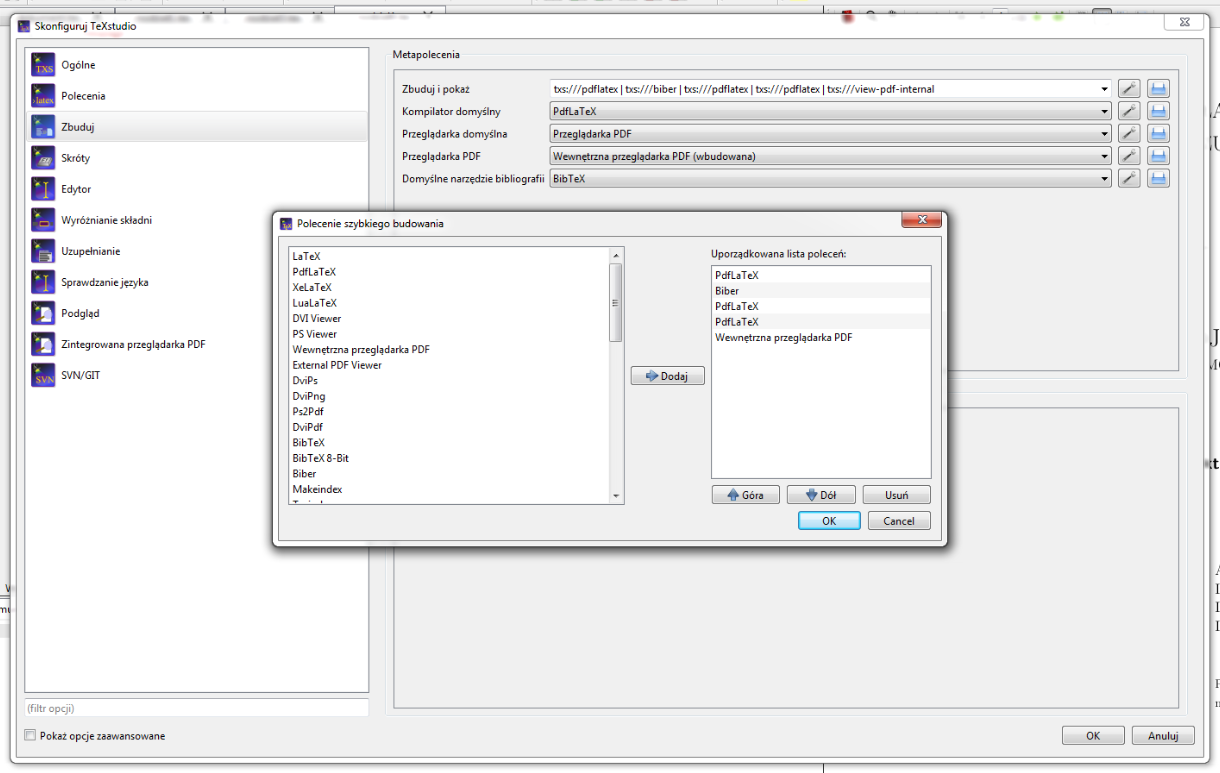
\includegraphics[width=\linewidth]{rys/ustawienie.png}
		\caption{Ustawienie TeXstudio}
		\label{rys:ustawienia}
	\end{center}
\end{figure}

Następnym krokiem jest ustawienie w \TeX{}Studio kolejności budowania projektu. Należy wybrać zakładkę: ,,Opcje/Konfiguruj \TeX{}studio...''. W otwartym oknie przechodzimy na zakładkę ,,Zbuduj''. Na rysunku \ref{rys:ustawienia} (s. \pageref{rys:ustawienia}) pokazany jest zrzut ekranu z konfiguracją. W linijce ,,Zbuduj i pokaż'' klikamy ikonę klucza, żeby przejść do konfiguracji polecenia. W otwartym oknie ustawić kolejność tak jak pokazano na rysunku.

 
 
 
 
 
\newpage
\section{Określenie wymagań szczegółowych}		%2
%Dokładne określenie wymagań aplikacji (cel, zakres, dane wejściowe) – np. opisać przyciski, czujniki, wygląd layautu, wyświetlenie okienek. Opisać zachowanie aplikacji – co po kliknięciu, zdarzenia automatyczne. Opisać możliwość dalszego rozwoju oprogramowania. Opisać zachowania aplikacji w niepożądanych sytuacjach.

\subsection{Cel aplikacji}
Celem aplikacji jest ułatwienie studentom oraz pracownikom uczelni dostępu do kluczowych funkcji administracyjnych i informacyjnych związanych z edukacją. Aplikacja ma zastąpić tradycyjne interakcje z dziekanatem, umożliwiając szybki dostęp do ocen, planu zajęć, harmonogramu egzaminów, e-dokumentów oraz ułatwiając komunikację z administracją uczelni.

\begin{itemize}
      \item \textbf{Zakres aplikacji:}
            \\\textbf{Studenci}: dostęp do ocen, planu zajęć, harmonogramu egzaminów, komunikacja z dziekanatem.
            \\\textbf{Wykładowcy/Pracownicy:} dostęp do harmonogramu zajęć, oceny studentów, komunikacja z dziekanatem.
            \\\textbf{Administracja: }zarządzanie danymi, kontakt ze studentami.
      \item \textbf{Platformy:}
            \\\textbf{Systemy operacyjne:} \\Android, \\iOS.
            \newpage
      \item \textbf{Dane wejściowe: (Logowanie użytkowników)}
            \\\textbf{Dane studentów}: nr indeksu, rocznik, oceny, plan zajęć, egzaminów, zgłoszenia do dziekanatu.
            \\\textbf{Zdarzenia dziekanatu}: zmiany w planie, ogłoszenia, nowe dokumenty, powiadomienia o ocenach.
            \\\textbf{Formularze zgłoszeń:} wnioski o zaświadczenia, prośby do dziekanatu.
      \item \textbf{Opis interfejsu użytkownika i elementów interaktywnych:}
            \\\textbf{Ekran logowania:}
            \\\textbf{Pola tekstowe:} „Email” oraz „Hasło”.
            \\\textbf{Przyciski:} „Zaloguj” – po kliknięciu, autoryzacja danych w tle i przejście do ekranu głównego. W przypadku błędnych danych, komunikat „Niepoprawne dane logowania”. „Zapomniałem hasła” – przekierowanie do formularza resetowania hasła.
      \item  \textbf{Ekran główny (Dashboard):}
            Wyświetlane informacje: skrót do ocen, nadchodzących zajęć, powiadomienia o ważnych wydarzeniach.
            \\\textbf{Przyciski:}
            \\\textbf{„Oceny”} – po kliknięciu, przejście do ekranu z listą ocen.
            \\\textbf{„Plan zajęć”} – po kliknięciu, podgląd planu zajęć (interaktywny kalendarz).
            \\\textbf{„Harmonogram egzaminów”} – otwiera harmonogram egzaminów z możliwością filtrowania według przedmiotu/semestru.
            \\\textbf{Automatyczne zdarzenia}: wyświetlanie powiadomień push o nadchodzących zajęciach, ocenach, ważnych wydarzeniach.
      \item \textbf{Ekran ocen:}
            \\\textbf{Tabela ocen:} kolumny „Przedmiot”, „Ocena”, „Komentarz wykładowcy”, „Data”.
            \\\textbf{Opcje sortowania}: sortowanie ocen po przedmiocie, dacie.
            \\\textbf{Zachowanie:} po kliknięciu w przedmiot, otwarcie szczegółów przedmiotu (np. opis, prowadzący, historia ocen).
            Plan zajęć:

      \item \textbf{Widok kalendarza}: wyświetlanie zajęć na dany tydzień/dzień.
            \\\textbf{Funkcje interaktywne}:
            \\Zmiana tygodnia za pomocą przesuwania palcem (swipe left/right).
            \\Kliknięcie na zajęcia otwiera szczegóły, np. nazwisko wykładowcy, sala, godziny.
            \\Powiadomienia push: automatyczne przypomnienia o nadchodzących zajęciach z możliwością wyłączenia.

      \item \textbf{Harmonogram egzaminów}:
            \\\textbf{Lista egzaminów}: możliwość filtrowania według przedmiotu, prowadzącego, daty.
            \\\textbf{Opcja zapisu}: jeśli wymagana rejestracja na egzamin, po kliknięciu „Zapisz się” użytkownik zapisuje się na egzamin.
            \\\textbf{Powiadomienia push}: przypomnienia o zbliżających się egzaminach.
            Komunikacja z dziekanatem:

      \item \textbf{Zdarzenia automatyczne}:
            \\Aplikacja będzie automatycznie wysyłać powiadomienia push o zmianach w planie zajęć, wynikach egzaminów, nowo dodanych dokumentach i ogłoszeniach.
            \\Automatyczne aktualizacje planu zajęć oraz harmonogramu egzaminów po synchronizacji z serwerem (np. co 30 minut).
      \item \textbf{Działanie offline}:
            \\Gdy brak połączenia z internetem, użytkownik ma dostęp do zapisanych wcześniej danych (plan zajęć, oceny).
      \item \textbf{Zachowanie aplikacji w niepożądanych sytuacjach}:
            \\\textbf{Brak połączenia z internetem:}
            \\Aplikacja wyświetla komunikat „Brak połączenia. Sprawdź połączenie z internetem” przy próbie wykonania operacji wymagającej synchronizacji z serwerem (np. wysłanie wiadomości do dziekanatu).
            W trybie offline: dostęp do zapisanych danych, brak możliwości interakcji z funkcjami wymagającymi połączenia.
            \\\textbf{Błędne dane logowania}:
            \\Komunikat „Niepoprawny email lub hasło” oraz możliwość ponownego wpisania danych. Pole tekstowe zostaje podświetlone na czerwono.
            \\\textbf{Serwer niedostępny}:
            \\Wyświetlenie komunikatu „Serwer dziekanatu jest obecnie niedostępny. Spróbuj ponownie później”.
            \\\textbf{Niepoprawne działanie aplikacji}:
            \\W przypadku błędu technicznego aplikacja wyświetli komunikat „Wystąpił błąd. Spróbuj ponownie” i zapisze logi błędów do późniejszej analizy przez programistów.
\end{itemize}

\newpage
\section{Projektowanie}		%3
%Opis przygotowania narzędzi (git, visual studio). Wybór i opis bibliotek, klas. Szkic layoutów. Pseudo kody. Opisy wykorzystanych algorytmów (np. algorytm sortowania). Dokładniejsze określenie założeń i działania aplikacji, (np.: ten przycisk otworzy takie okno a w tym oknie wpisujemy takie dane).

W ramach przygotowania środowiska do implementacji aplikacji wirtualnego dziekanatu oraz zarządzania wersjami kodu, wybrano zestaw narzędzi wspierających proces tworzenia oraz zapewniających automatyzację wielu czynności. W poniższych punktach opisano każde z wykorzystanych narzędzi wraz z ich rolą oraz załączonym linkiem do dokumentacji.

\subsection{Przygotowanie narzędzi}

\begin{itemize}
  \item \textbf{Git} – system kontroli wersji, umożliwiający śledzenie zmian w kodzie oraz współpracę w zespole. Dokumentacja narzędzia: \url{https://git–scm.com/doc}
  \item \textbf{VSCode} – edytor kodu źródłowego, który zapewnia wsparcie dla wielu języków programowania i umożliwia instalację rozszerzeń wspierających programowanie. Dokumentacja narzędzia: \url{https://code.visualstudio.com/docs}
  \item \textbf{Doxygen} – narzędzie do generowania dokumentacji automatycznej na podstawie komentarzy w kodzie źródłowym. Ułatwia utrzymywanie aktualnej dokumentacji technicznej. Dokumentacja narzędzia: \url{https://www.doxygen.nl/}
  \item \textbf{Doxygen Awesome} – motyw graficzny dostosowujący wygląd strony wygenerowanej przez Doxygen do współczesnych standardów. Motyw jest zainspirowany stroną Nuxt i pomaga poprawić czytelność dokumentacji. Więcej informacji: \url{https://github.com/jothepro/doxygen–awesome–css}
  \item \textbf{Lefthook} – narzędzie do zarządzania hookami Git, które wspiera automatyczne formatowanie, walidację kodu, generowanie dokumentacji oraz zgodność wiadomości commitów z konwencją. Dokumentacja narzędzia: \url{https://github.com/evilmartians/lefthook}
  \item \textbf{Commitlint} – narzędzie do sprawdzania zgodności wiadomości commitów z konwencją \textit{Conventional Commits}. Dokumentacja: \url{https://commitlint.js.org/}
  \item \textbf{GitHub Actions} – platforma do automatyzacji procesów CI/CD. Umożliwia między innymi automatyczną walidację commitów, generowanie dokumentacji oraz wersjonowanie wydań. Dokumentacja: \url{https://docs.github.com/en/actions}
\end{itemize}

\subsection{Wybór technologii}

\subsection{Framework Flutter}

Flutter to framework stworzony przez Google, umożliwiający tworzenie aplikacji wieloplatformowych z jednego kodu źródłowego, co znacząco skraca czas potrzebny na rozwój aplikacji. W projekcie wirtualnego dziekanatu Flutter został wybrany ze względu na jego elastyczność oraz bogaty ekosystem widgetów. Poniżej przedstawiono kluczowe aspekty wykorzystania Fluttera w projekcie.

\begin{itemize}
  \item \textbf{Material Design} – Flutter dostarcza szeroką gamę komponentów zgodnych z wytycznymi Material Design, co pozwala na stworzenie nowoczesnego i spójnego interfejsu użytkownika, dostosowanego do standardów Google. Dokumentacja: \url{https://flutter.dev/docs/development/ui/widgets/material}
  \item \textbf{Hot Reload} – Flutter umożliwia szybkie testowanie zmian w kodzie dzięki funkcji Hot Reload, która natychmiast odświeża widoki aplikacji, co pozwala programistom na szybką iterację i oszczędność czasu w trakcie testowania.
  \item \textbf{Kompatybilność wieloplatformowa} – Aplikacja wirtualnego dziekanatu została zaprojektowana jako aplikacja mobilna, ale Flutter umożliwia łatwe rozszerzenie wsparcia na inne platformy, takie jak web, desktop (Windows, macOS, Linux) oraz urządzenia IoT.
  \item \textbf{State Management (Zarządzanie stanem)} – W projekcie zastosowano zarządzanie stanem z użyciem pakietu Provider, co umożliwia łatwe zarządzanie danymi oraz stanami ekranów, szczególnie w dynamicznych sekcjach, takich jak ekran wiadomości czy plan zajęć. Dokumentacja Provider: \url{https://pub.dev/packages/provider}
  \item \textbf{Bogaty ekosystem pakietów} – Flutter wspiera szeroką gamę pakietów dostępnych w repozytorium \texttt{pub.dev}, co pozwala na szybkie wdrożenie dodatkowych funkcji. Przykłady wykorzystanych pakietów to:
        \begin{itemize}
          \item \textbf{firebase\_auth} – zapewnia integrację z Firebase Authentication dla bezpiecznego logowania użytkowników. Dokumentacja: \url{https://pub.dev/packages/firebase_auth}
          \item \textbf{cloud\_firestore} – pozwala na połączenie z bazą danych Firestore i zarządzanie danymi w czasie rzeczywistym. Dokumentacja: \url{https://pub.dev/packages/cloud_firestore}
          \item \textbf{firebase\_messaging} – umożliwia wysyłanie powiadomień push do użytkowników. Dokumentacja: \url{https://pub.dev/packages/firebase_messaging}
          \item \textbf{intl} – używany do formatowania dat i liczb, co wspiera różne lokalizacje i języki. Dokumentacja: \url{https://pub.dev/packages/intl}
        \end{itemize}
  \item \textbf{Wysoka wydajność} – Flutter jest bezpośrednio kompilowany do natywnego kodu ARM, co zapewnia wydajność zbliżoną do natywnych aplikacji. Dla płynnego działania aplikacji kluczowe było odpowiednie zarządzanie wydajnością komponentów i optymalizacja ekranów, szczególnie dla list z dużą ilością danych, jak np. plan zajęć.
  \item \textbf{Testy jednostkowe i widgetowe} – Flutter oferuje rozbudowane wsparcie dla testów, co umożliwia testowanie logiki biznesowej aplikacji (testy jednostkowe) oraz interakcji użytkownika z komponentami UI (testy widgetowe). Dzięki temu można łatwo wykrywać błędy i sprawdzać działanie aplikacji w sposób automatyczny.
\end{itemize}

\subsection{Wykorzystane biblioteki Flutter}
\begin{itemize}
  \item \textbf{Riverpod} – zaawansowany pakiet do zarządzania stanem aplikacji. Dokumentacja: \url{https://pub.dev/packages/flutter_riverpod}
  \item \textbf{Google Nav Bar} – pakiet do tworzenia nawigacji dolnej w aplikacji. Dokumentacja: \url{https://pub.dev/packages/google_nav_bar}
  \item \textbf{Table Calendar} – interaktywny kalendarz do wyświetlania planu zajęć. Dokumentacja: \url{https://pub.dev/packages/table_calendar}
  \item \textbf{Wirtualny SDK} – własny moduł SDK do komunikacji z własnym backendem.
  \item \textbf{Firebase Messaging} – moduł do wysyłania powiadomień push do użytkowników. Dokumentacja: \url{https://firebase.google.com/docs/cloud–messaging}
  \item \textbf{Shared Preferences} – przechowywanie danych lokalnych w aplikacji. Dokumentacja: \url{https://pub.dev/packages/shared_preferences}
  \item \textbf{Image Picker} – wybieranie obrazów z galerii lub aparatu. Dokumentacja: \url{https://pub.dev/packages/image_picker}
  \item \textbf{URL Launcher} – otwieranie linków w przeglądarce. Dokumentacja: \url{https://pub.dev/packages/url_launcher}
  \item \textbf{Flutter Chat UI} – interfejs użytkownika dla funkcji czat. Dokumentacja: \url{https://pub.dev/packages/flutter_chat_ui}
  \item \textbf{UUID} – generowanie unikalnych identyfikatorów. Dokumentacja: \url{https://pub.dev/packages/uuid}
  \item \textbf{HTTP} – obsługa żądań HTTP. Dokumentacja: \url{https://pub.dev/packages/http}
  \item \textbf{Intl} – formatowanie dat i liczb, wspierające różne lokalizacje i języki. Dokumentacja: \url{https://pub.dev/packages/intl}
  \item \textbf{Flutter Launcher Icons} – generowanie ikon aplikacji. Dokumentacja: \url{https://pub.dev/packages/flutter_launcher_icons}
  \item \textbf{Flutter Localization} – wsparcie dla lokalizacji aplikacji. Dokumentacja: \url{https://pub.dev/packages/flutter_localization}
\end{itemize}

	\newpage
\section{Implementacja}		%4
%Wkleić szkielet kodu, wraz z komentarzami. Opisać zmienne, struktury do czego służą. Opisać procedury, metody co wykonują. Opisać nowe zdefiniowane klasy. Opisać dziedziczenie. Opisać nowo utworzone pliki za co odpowiadają.




	\newpage
\section{Testowanie}	%5
%Opisujemy testy, sprawdzamy czy nie generuje błędów.



	\newpage
\section{Podręcznik użytkownika}  %6
%Opis jak używać programu. Mogą być z zrzut ekranu razem z opisem. 




%%%%%%%%%%%%%%%%%%% koniec treść główna dokumentu %%%%%%%%%%%%%%%%%%%%%
\newpage
\addcontentsline{toc}{section}{Literatura}
\printbibliography{}

\newpage
\hypersetup{linkcolor=black}
\renewcommand{\cftparskip}{3pt}
\clearpage
\renewcommand{\cftloftitlefont}{\Large\bfseries\sffamily}
\listoffigures
\addcontentsline{toc}{section}{Spis rysunków}
\thispagestyle{fancy}

\newpage
\renewcommand{\cftlottitlefont}{\Large\bfseries\sffamily}
\def\listtablename{Spis tabel}
\addcontentsline{toc}{section}{Spis tabel}\listoftables
\thispagestyle{fancy}

\newpage
\renewcommand{\cftlottitlefont}{\Large\bfseries\sffamily}
\renewcommand\lstlistlistingname{Spis listingów}
\addcontentsline{toc}{section}{Spis listingów}\lstlistoflistings{}
\thispagestyle{fancy}



%lista rzeczy do zrobienia: wypisuje na koñcu dokumentu, patrz: pakiet todo.sty
\todos{}
%koniec listy rzeczy do zrobienia
\end{document}
